\chapter*{Making sense of data}
\addcontentsline{toc}{chapter}{Making sense of dataset}
\setcounter{section}{0}
\renewcommand*{\theHsection}{ch1.\the\value{section}}

\section{Data categorization}

An \emph{observational unit} is the person or thing on which measurements are
taken. Note that this can also be a case, object, a subject and so on. A
\emph{variable} is a characteristic measured on the observational unit. An
instance of the variable we call the \emph{observed value} or
\emph{observation}. Variables can be of three kind:

\begin{description}
  \item[quantitive] variable take numerical values for which arithmetic
  operations make sense. The height of the people is a such variable,
  \item[caterogical] variable consist of records into which the observation
  falls into (one of several categories). For example the countries of the
  world may be classified into one of the five great continets: Europe, America,
  Africa, Asia and the Pacific,
  \item[ordinal] variable have natural order, however the difference between two
  instance of the variables does nt always make sense. A good example is grades
  given by a teacher: A, B, C, D, E, F.
   
\end{description}

\section{Quantative variables}

One way of making sense of a quantitive variable is to use the \emph{five
number summary}. Given a collection of a observations we can calculate the: 

\begin{description}
  \item[Minimum] is the lowest observation value.
  \item[Maximum] is the highest observation value.
  \item[Median] is the center observation, average point. To find it you'll need
  to sort the observations, and then take the observation in the middle
  position.
  \item[First quartile] is the observation value at the $\frac{1}{4}$rd position
  in the sorted observation array.
  \item[Third quartile] is the observation value at the $\frac{3}{4}$rd position
  in the sorted observation array.
\end{description}

A graphical representation of this five values is possible via the
\emph{boxplot} as shown on figure \ref{fig:boxplot}. On the boxplot the whiskers
show the minimum and the maximum values.

\begin{figure}[htbp]
\label{fig:boxplot}
\caption{A simple way to represent the \emph{five number summary}.}
\includegraphics{1/boxplot-boxplot}
\end{figure}

Note that the median, first or thrid quartile may result in a non--integer
position. In this case these values are calcualted by interpolating them from
the nearby observations, with the given percentage; therefore, it may happen that
these values are not part of the variable instances.

\subsection{Modified boxplots}
Outliers (known as extreme values, or unusual observations) are hard
to study on a classical boxplot, so for them we use the modified boxplot. In
this case let us first define the inter-quartile range (noted as \emph{IQR}) as
the difference between the $3$rd and the $1$st quartile. Then we can define the
inner fences as the:

\begin{description}
  \item[lower fence]  is $=1$st quartile $- ~1.5\cdot $IQR, and the  
  \item[upper fence]  is $=3$st quartile $+ ~1.5\cdot $IQR.  
\end{description}

Now the lower whisker is noted as the lower fence, while the upper fence as the
upper whisker. Observations smaller than the lower fence, or larger than the
upper fence are drawn with their own circle on the plot as shown on figure
\ref{fig:boxplot_modified}.

\begin{figure}[htbp]
\label{fig:boxplot_modified}
\caption{Modified boxplots help dealing with outliers.}
\includegraphics{1/boxplot_modified-boxplot_modified}
\end{figure}

\subsection{Mean}
Given a list of observations ($x_1, x_2, \ldots x_n$), the mean of the variable
is noted as $\bar{x}$ (or $\mu$) and is calculated as: 
\[ \mbox{Mean} = \bar{x} = 
\frac{\sum{\mbox{data values}}}{\mbox{number of data points}} =
\frac{\sum_{i=1}^{n}{x_i}}{n}.
\]

However, this definition of mean is not robust, as it's easily influenced by
outlier points. Note, that in contrast the median is robust. To alleviate this
we can introduce the conept of trimmed mean, which exclude some percentage of
the lowest and highest values from the observations, before performing the same
operation to calculate the \emph{trimmed--mean}. The input of the trimmed mean
is the percentage of outliers to remove. 

\subsection{Spread of the data}

The range of the data is the difference between the maximum and the minimum.
This is not a robust measurement. The same can be told about the IQR too. The
deviation of an observation $i$ is $x_i - \bar{x}$. A good show of the spread of
the whole data is the:

\[ \mbox{variance} = \frac{\sum_{i=1}^{n}\left(x_i - \bar{x} \right)^2}{n-1}
\]

Note that we divide by one less than the count of observation points. An
intuitive explanation for this is that the first observation does not tells us
anything about deviation. The \emph{standard deviation} (also noted as $\sigma$)
is the square root of this ($\sqrt{\mbox{variance}}$), and shows the dispersion of a set of data from
its mean.

\subsection{The shape of the data - histogram}

\begin{figure}[htbp]
\label{fig:histogram}
\caption{Histogram}
\includegraphics{1/histogram-histogram}
\end{figure}

The distribution is the pattern of values in the data, showing their frequency
of occurance relative to each other. The histogram is a good way to show this
graphically; you can see an example of this on figure \ref{fig:histogram}.

Its key part is the number of \emph{bin}s used, as observations must be
separated into mutually exclusive and exhaustive bins. \emph{Cutpoints} define
where the bins start and where they end. Each bin has its own \emph{frequency},
the number of observations in it. The largest bins define the \emph{peaks} or 
\emph{modes}. If a variable has a single peak we call it an unimodal, bimodal
for two peaks and multiple peaks above that.

\begin{figure}[htbp]
\label{fig:histogram_skewed}
\caption{Skewed histograms}
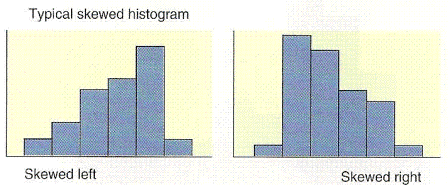
\includegraphics{img/skewed.png}
\end{figure}

Uniform distribution is a case when all the data values occur around the same
times, so we have no peaks, and such the variable has no mode. The tails of the
histogram are on its left or right side, where its extreme values are. A
histogram is left skewed if it has the left tail larger than the right, and
right skewed if the right tail  is larger than its left. 

\subsection{Empirical rule}

The empirical rule (also know as three $\sigma$ rule) states that for a normal
distribution $68\%$ of the data is within one standard deviation of the mean
value, $95\%$ is within two standard deviation, and $99.7\%$ is within three
standard deviation.

\section{Categorical variables}

Caterogical variables are not represented by numbers, so all of the earlier
statistics no longer make sense. What does make sense is the frequency of the
categories, which is graphically represented either by a barchart or a piechart.

Figure \ref{fig:category_representation} shows an example of this. In case of
barcharts we may choose to normalize the frequency, by dividing it with the
total number of observations.

\begin{figure}[htbp]
\label{fig:category_representation}
\caption{Skewed histograms}
\includegraphics{1/categorical_representation-categorical_representation}
\end{figure}